\section{Auswertung}
\label{sec:Auswertung}
Es werden die Bremsspannungen $U_{\symup{B}}$ gegen die Wurel des Photostroms $\sqrt{I}$ für die
rote, gelbe, grüne und violette Spektrallinie aufgetragen und mit Hilfe einer durch
Python berechneten Ausgleichsgeraden die Grenzspannung $U_G$ bestimmt.\\
\\
Die Messwerte für die rote Spektrallinie sind in \autoref{tab:rot}, die für die gelbe in \autoref{tab:gelb},
die für die grüne in \autoref{tab:gruen} und die der ersten violetten in \autoref{tab:violett1} zu finden.
Für die zweite violette Spektrallinie konnten keine Messwerte aufgenommen werden, da die Versuchsappartatur
beschädigt war.
\begin{table}[H]
    \centering
    \caption{Messwerte für die rote Spektrallinie.}
    \label{tab:rot}
    \begin{tabular}{c c}
        \toprule
        $U_{\symup{B}} / \unit{\milli\volt}$ & $I / \unit{\nano\ampere}$ \\
        \midrule
          0 & 0,040 \\
         20 & 0,030 \\
         40 & 0,025 \\
         60 & 0,020 \\
         80 & 0,020 \\
        100 & 0,020 \\
        120 & 0,020 \\
        220 & 0,010 \\
        380 & 0,000 \\
        \bottomrule
    \end{tabular}
\end{table}

\begin{table}[H]
    \centering
    \caption{Messwerte für die gelbe Spektrallinie.}
    \label{tab:gelb}
    \begin{tabular}{c c}
        \toprule
        $U_{\symup{B}} / \unit{\milli\volt}$ & $I / \unit{\nano\ampere}$ \\
        \midrule
         0 & 1,000 \\
        20 & 0,900 \\
        40 & 0,810 \\
        60 & 0,720 \\
        80 & 0,640 \\
       100 & 0,550 \\
       120 & 0,475 \\
       140 & 0,400 \\
       160 & 0,350 \\
       180 & 0,290 \\
       200 & 0,230 \\
       220 & 0,190 \\
       240 & 0,150 \\
       260 & 0,100 \\
       280 & 0,100 \\
       300 & 0,090 \\
       320 & 0,060 \\
       340 & 0,050 \\
       360 & 0,040 \\
       380 & 0,010 \\
       400 & 0,010 \\
       420 & 0,005 \\
       440 & 0,000 \\
        \bottomrule
    \end{tabular}
\end{table}

\begin{table}[H]
    \centering
    \caption{Messwerte für die grüne Spektrallinie.}
    \label{tab:gruen}
    \begin{tabular}{c c}
        \toprule
        $U_{\symup{B}} / \unit{\milli\volt}$ & $I / \unit{\nano\ampere}$ \\
        \midrule
          0 & 5,00 \\
         20 & 4,90 \\
         40 & 4,80 \\
         80 & 3,80 \\
        120 & 3,00 \\
        160 & 2,40 \\
        200 & 1,80 \\
        240 & 1,25 \\
        280 & 0,90 \\
        320 & 0,60 \\
        360 & 0,40 \\
        400 & 0,20 \\
        440 & 0,10 \\
        480 & 0,00 \\
        \bottomrule
    \end{tabular}
\end{table}

\begin{table}[H]
    \centering
    \caption{Messwerte für die erste violette Spektrallinie.}
    \label{tab:violett1}
    \begin{tabular}{c c}
        \toprule
        $U_{\symup{B}} / \unit{\milli\volt}$ & $I / \unit{\nano\ampere}$ \\
        \midrule
          0 & 5,50 \\
         40 & 4,80 \\
         80 & 4,20 \\
        120 & 3,60 \\
        160 & 3,20 \\
        200 & 2,80 \\
        240 & 2,60 \\
        280 & 2,20 \\
        320 & 1,90 \\
        360 & 1,75 \\
        400 & 1,60 \\
        440 & 1,40 \\
        480 & 1,20 \\
        520 & 1,00 \\
        560 & 0,80 \\
        600 & 0,60 \\
        640 & 0,50 \\
        680 & 0,40 \\
        720 & 0,30 \\
        760 & 0,10 \\
        800 & 0,10 \\
        840 & 0,05 \\
        880 & 0,00 \\
        \bottomrule
    \end{tabular}
\end{table}

Die Plots mit den entsprechenden linearen Regressionen für rot, gelb, grün und violett sind in Abbildung 6,
Abbildung 7, Abbildung 8 und Abbildung 9 zu finden.
\begin{figure}[H]
    \centering
    \label{fig:rot}
    \caption{Photostrom in Abhängigkeit der Bremsspannung und Ausgleichsgerade für die rote Spektrallinie.}
    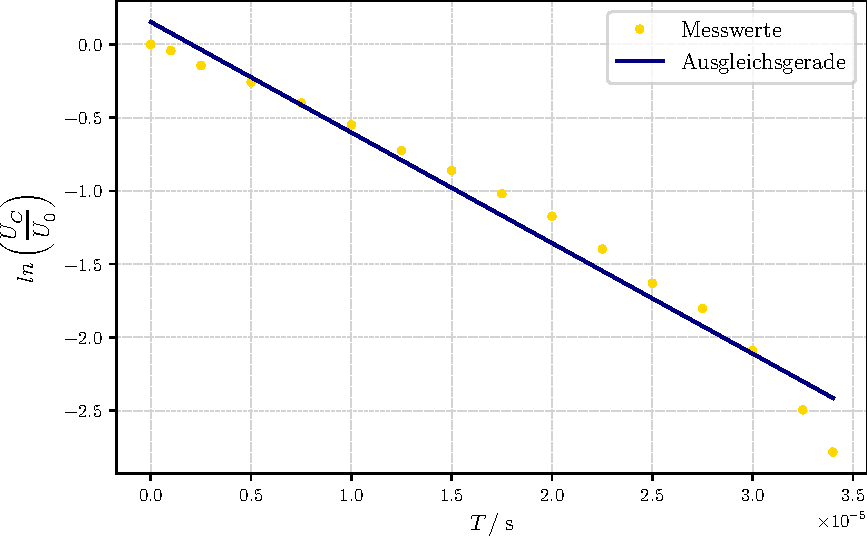
\includegraphics[width=\textwidth]{plot1.pdf}
\end{figure}

\begin{figure}[H]
    \centering
    \label{fig:gelb}
    \caption{Photostrom in Abhängigkeit der Bremsspannung und Ausgleichsgerade für die gelbe Spektrallinie.}
    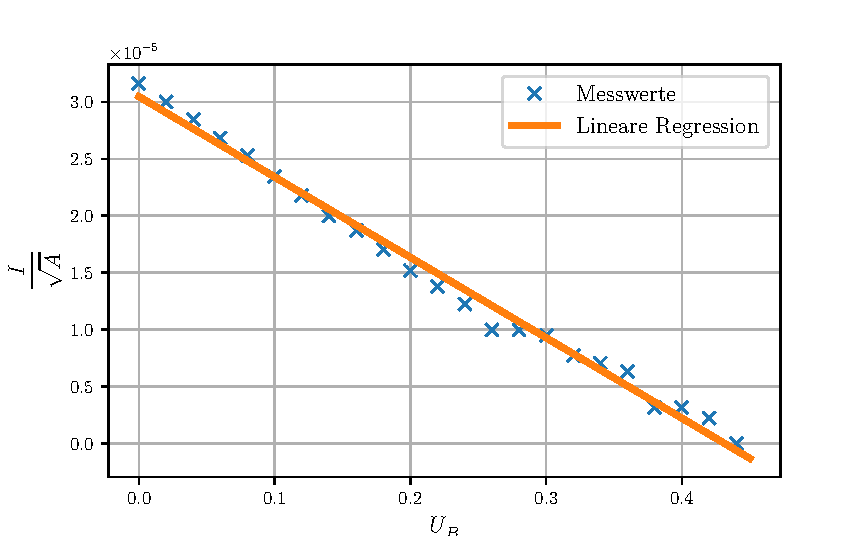
\includegraphics[width=\textwidth]{plot2.pdf}
\end{figure}


\begin{figure}[H]
    \centering
    \label{fig:gruen}
    \caption{Photostrom in Abhängigkeit der Bremsspannung und Ausgleichsgerade für die grüne Spektrallinie.}
    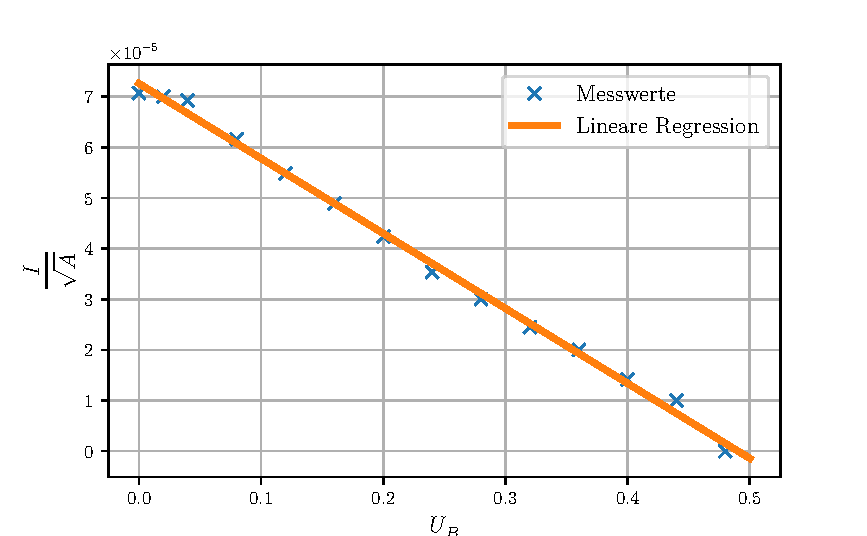
\includegraphics[width=\textwidth]{plot3.pdf}
\end{figure}

\begin{figure}[H]
    \centering
    \label{fig:violett1}
    \caption{Photostrom in Abhängigkeit der Bremsspannung und Ausgleichsgerade für die erste violette Spektrallinie.}
    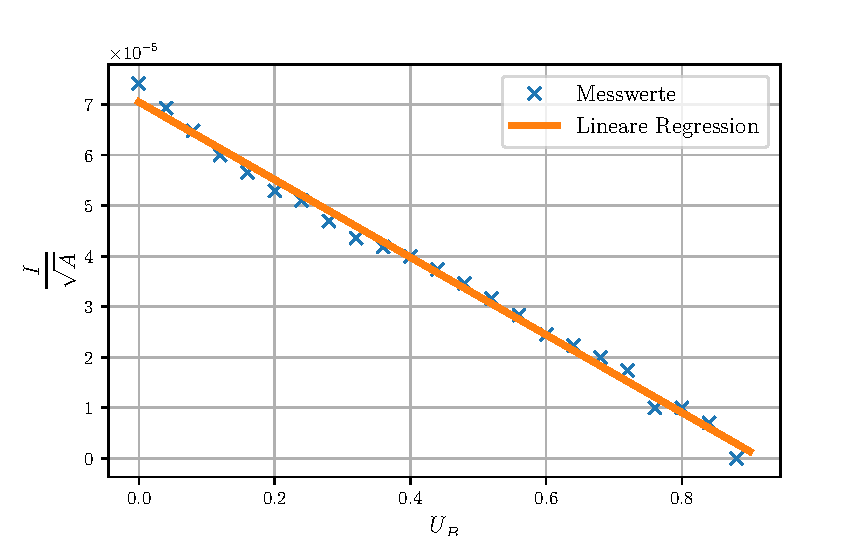
\includegraphics[width=\textwidth]{plot4.pdf}
\end{figure}

\subsection{Grenzspannung}
\label{sec:Grenzspannung}
Die Ausgleichsgerade hat die Form $\sqrt{I} = a \cdot U_{\symup{B}} + b$. Die Grenzspannung $U_{\symup{G}}$
ergibt sich aus dem Verhältnis $\frac{-b}{a}$. Die für $a$ und $b$ bestimmten Werte und die Grenzspannung
$U_{\symup{G}}$ sind in Tabelle 5 eingetragen.
\begin{table}[H]
    \centering
    \label{tab:UG}
    \caption{Werte der linearen Regression.}
    \begin{tabular}{c c c c}
        \toprule
        $\lambda/\unit{\nano\meter}$ & $a\cdot 10^{-5}$ & $b\cdot 10^{-5}$ & $U_{\symup{G}}/\unit{\volt}$\\
        \midrule
        646 &  -1,47 $\pm$ 0,12 & 0,59 $\pm$ 0,02 & 0,401 $\pm$ 0,035 \\
        578 &  -7,06 $\pm$ 0,15 & 3,05 $\pm$ 0,04 & 0,432 $\pm$ 0,011 \\
        546 & -14,81 $\pm$ 0,26 & 7,26 $\pm$ 0,07 & 0,490 $\pm$ 0,010 \\
        435 &  -7,68 $\pm$ 0,14 & 7,05 $\pm$ 0,07 & 0,981 $\pm$ 0,019 \\
        \bottomrule
    \end{tabular}
\end{table}

\subsection{Plancksche Wirkungsquantum}
\label{sec:Plancksche_Wirkungsquantum}
Nun wird die Grenzspannung in \autoref{fig:Uf} gegen die Frequez des Lichts aufgetragen.
\begin{figure}[H]
    \centering
    \caption{Grenzspannung gegen die Frequenz aufgetragen mit linearer Regression.}
    \label{fig:Uf}
    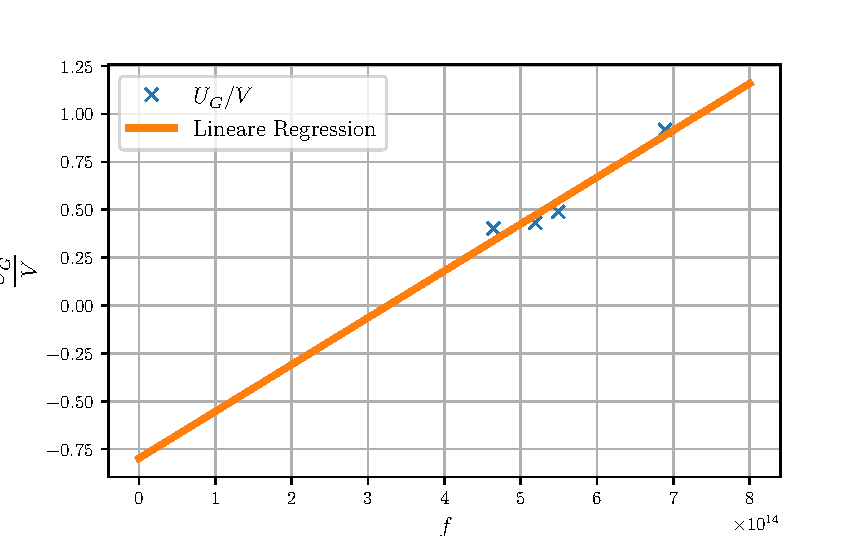
\includegraphics[width=\textwidth]{plot5.pdf}
\end{figure}
Aus der linearen Regression und \autoref{eqn:1und2} ergibt sich $a=\frac{h}{e_{\symup{0}}}$ und
$b=A_{\symup{k}}$. Die Werte ermitteln sich zu
\begin{align*}
    \frac{h}{e_{\symup{0}}}&= (2,4 \pm 0,4)\cdot 10^{-15}\unit{\volt\second}\\
    A_{\symup{k}} &= (0,80 \pm 0,23) e\unit{\volt}.\\
\end{align*}

\subsection{Kurvenverlauf}
\label{sec:Kurvenverlauf}
In \autoref{fig:kurve} ist der Photostrom gegen die Brems- bzw. Beschleunigungsspannung von ca.
$-12\unit{\volt}$ bis $0,2\unit{\volt}$ aufgetragen.
\begin{figure}[H]
    \centering
    \caption{Photostrom in Abhängigkeit der Spannung für die gelbe Spektrallinie.}
    \label{fig:kurve}
    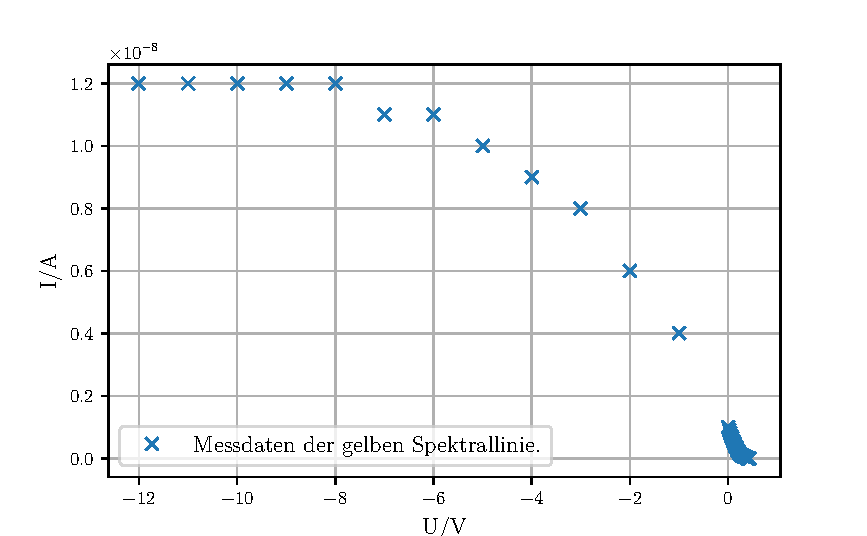
\includegraphics[width=\textwidth]{plot6.pdf}
\end{figure}
Die Kurve entspricht den Erwartungen. Für hohe Beschleunigungsspannungen nähert sich die Kurve asymptotisch
einem Sättigungswert an. Für Spannungen die gegen die Grenzspannung $U_{\symup{G}}$ gehen, geht der Photostrom
gegen Null. Dieser Umstand lässt sich dadurch erklären, dass die Elektronen energetisch verteilt sind und deshalb
schon bei $U<U_{\symup{G}}$ sich Null annähern. Da die Lichtintensität konstant ist, kann nur eine begrenzte
Anzahl von Elektronen losgelöst werden, so dass die Kurve sich einem Sättigungswert annähert.